 \documentclass{article}
\usepackage{graphicx}
\usepackage[T1]{fontenc}
\graphicspath{ {./images/} }
\usepackage[utf8]{inputenc}
\usepackage{hyperref}
\usepackage{amsmath}
\usepackage{footnotebackref}
%\usepackage[symbol=$\wedge$]{footnotebackref}
%\usepackage[numberlinked=false]{footnotebackref}
\usepackage{a4wide}

\title{Project proposal (extended)}
\author{Antoni Dąbrowski, Cezary Troska}
\date{\today}

\begin{document}
\maketitle
\section{Project plan}
We will explore the field of language modeling for the authorship identification task. We are going to test a new, proposed by us pre-training procedure on few existing models. The main idea of this method is to train feature extracting model on different book translations to guide it into a deeper understanding of language model - focusing on style, sentiment and syntax analysis, rather than text subject itself.

\section{Hypotheses}
\begin{enumerate}
    \item Using our pre-training method will decrease amount of text needed to predict its author.
    \item Developed during the process of pre-training the feature extracting model will provide new, valuable information to standard authorship identification algorithms, that will lead to achieving better results.
\end{enumerate}

\section{Motivation}
Classical algorithms in general are trained on texts that are fundamentally different. Both in term of content and character. Therefore it could be hard or even impossible task for them to fully understand how one and the other component is related to an author. Our pre-training procedure will provide a model that is ``blind to'' the subject and can distinguish very subtle differences in style. For that reason we believe that proposed method might be beneficial.

\section{Testing hypotheses}
Process of testing the hypotheses will consist two stages. Firstly we are going to perform learning procedure on different translations of a book to get feature extracting model (\textbf{FE}). Secondly we are going to use it in real task. Specifically, we are going to take new data containing different texts of different authors (not translations) and we will split it into training and testing sets. Then we will train models [Figure 3], [Figure 4] and measure their performance. Validation will require collecting error rates for each given text length. Comparison of the result of models [Figure 3] and [Figure 4] will let us answer whether our hypothesis were right.

\section{Models}
\subsection{Pre-training}
Main goal of this phase is to get a \textbf{FE} that will create reasonable text embeddings. We see two methods that are promising.

\begin{figure}
  \centering
        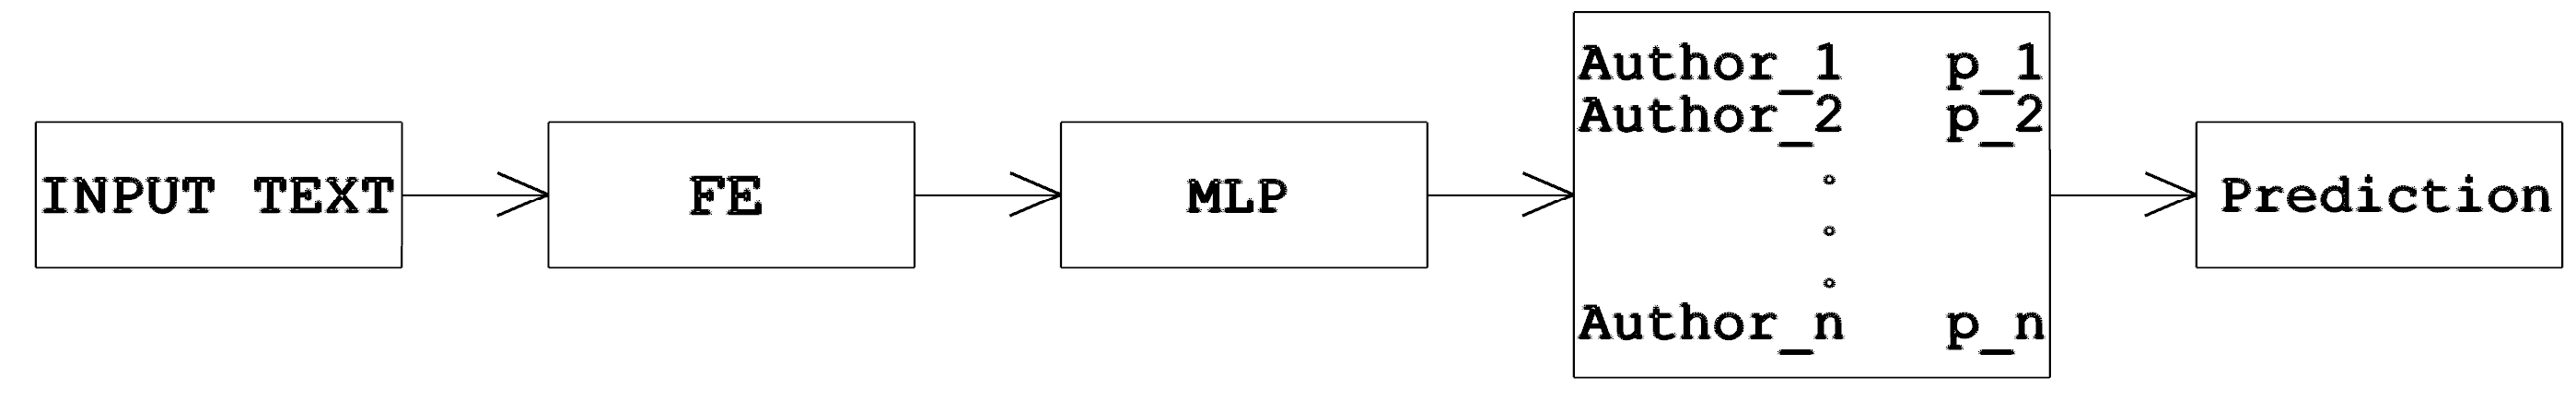
\includegraphics[width=0.8\textwidth]{Simple_model.png}
        \caption{Chunks of texts (e.g. paragraphs) will pass through \textbf{FE}. Then received embedding is given to a classification model which tries to identify author.}
\end{figure}

\textbf{Simple model} - Figure 1. In principle this model should learn how to distinguish between different language models tied with translators not by text content, but by way of describing it. Simplicity of this architecture should make learning procedure fast and stable.

\begin{figure}
  \centering
        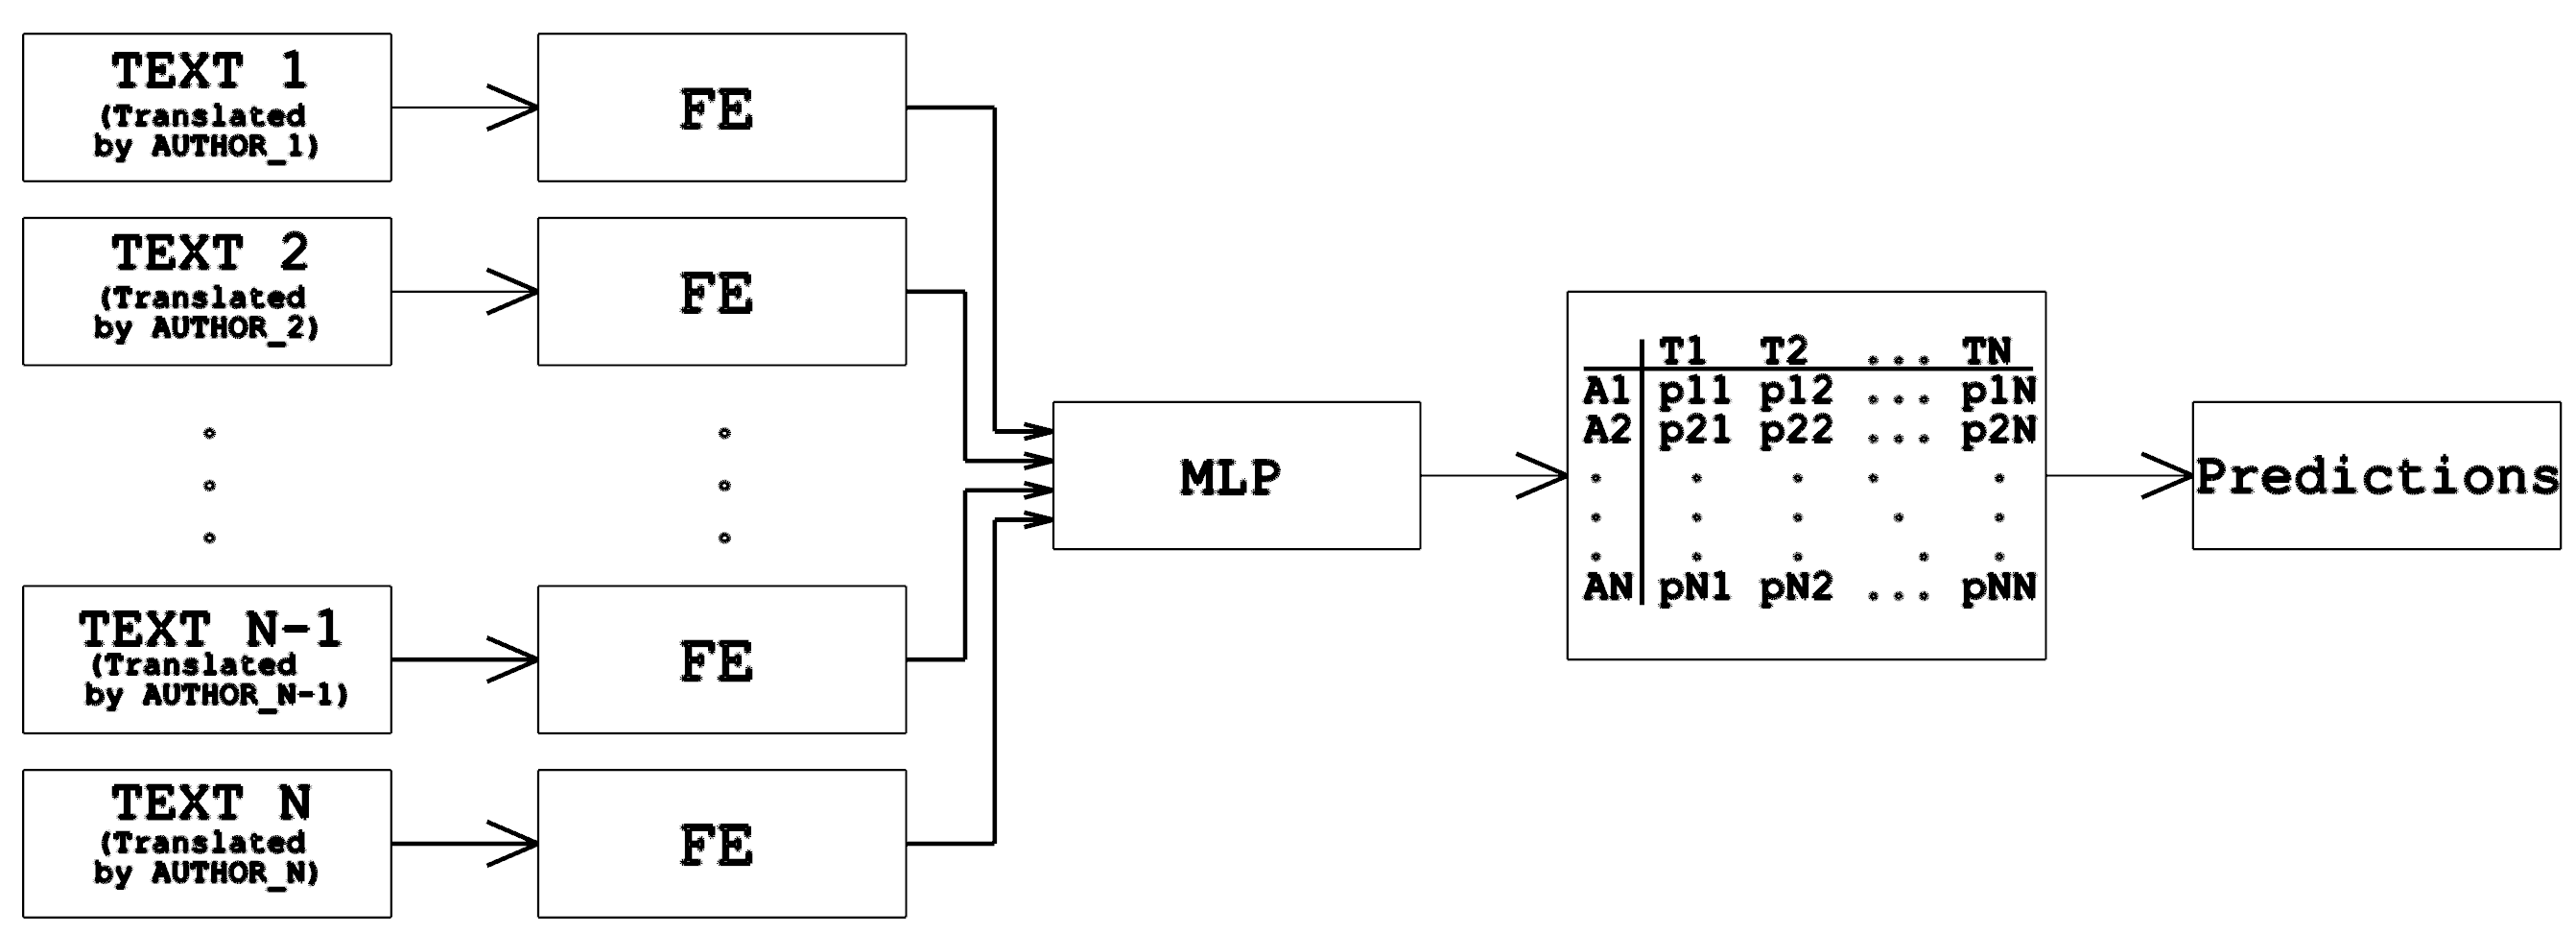
\includegraphics[width=0.8\textwidth]{Complex_model.png}
        \caption{Chunks of different translations (e.g. paragraphs) will in parallel pass through the same \textbf{FE} (in terms of architecture and parameters). Then received embeddings is given to classification model that for each input text will produce vector of author probabilities.}
\end{figure}

\textbf{Complex model} - Figure 2. This model aims to force even harder \textbf{FE} into understanding author style by exposing it to different translations of the same text at once. 

\subsection{Application}
Application of our \textbf{FE} will be done as described previously using models from Figure 3 and 4.
\begin{figure}
  \centering
        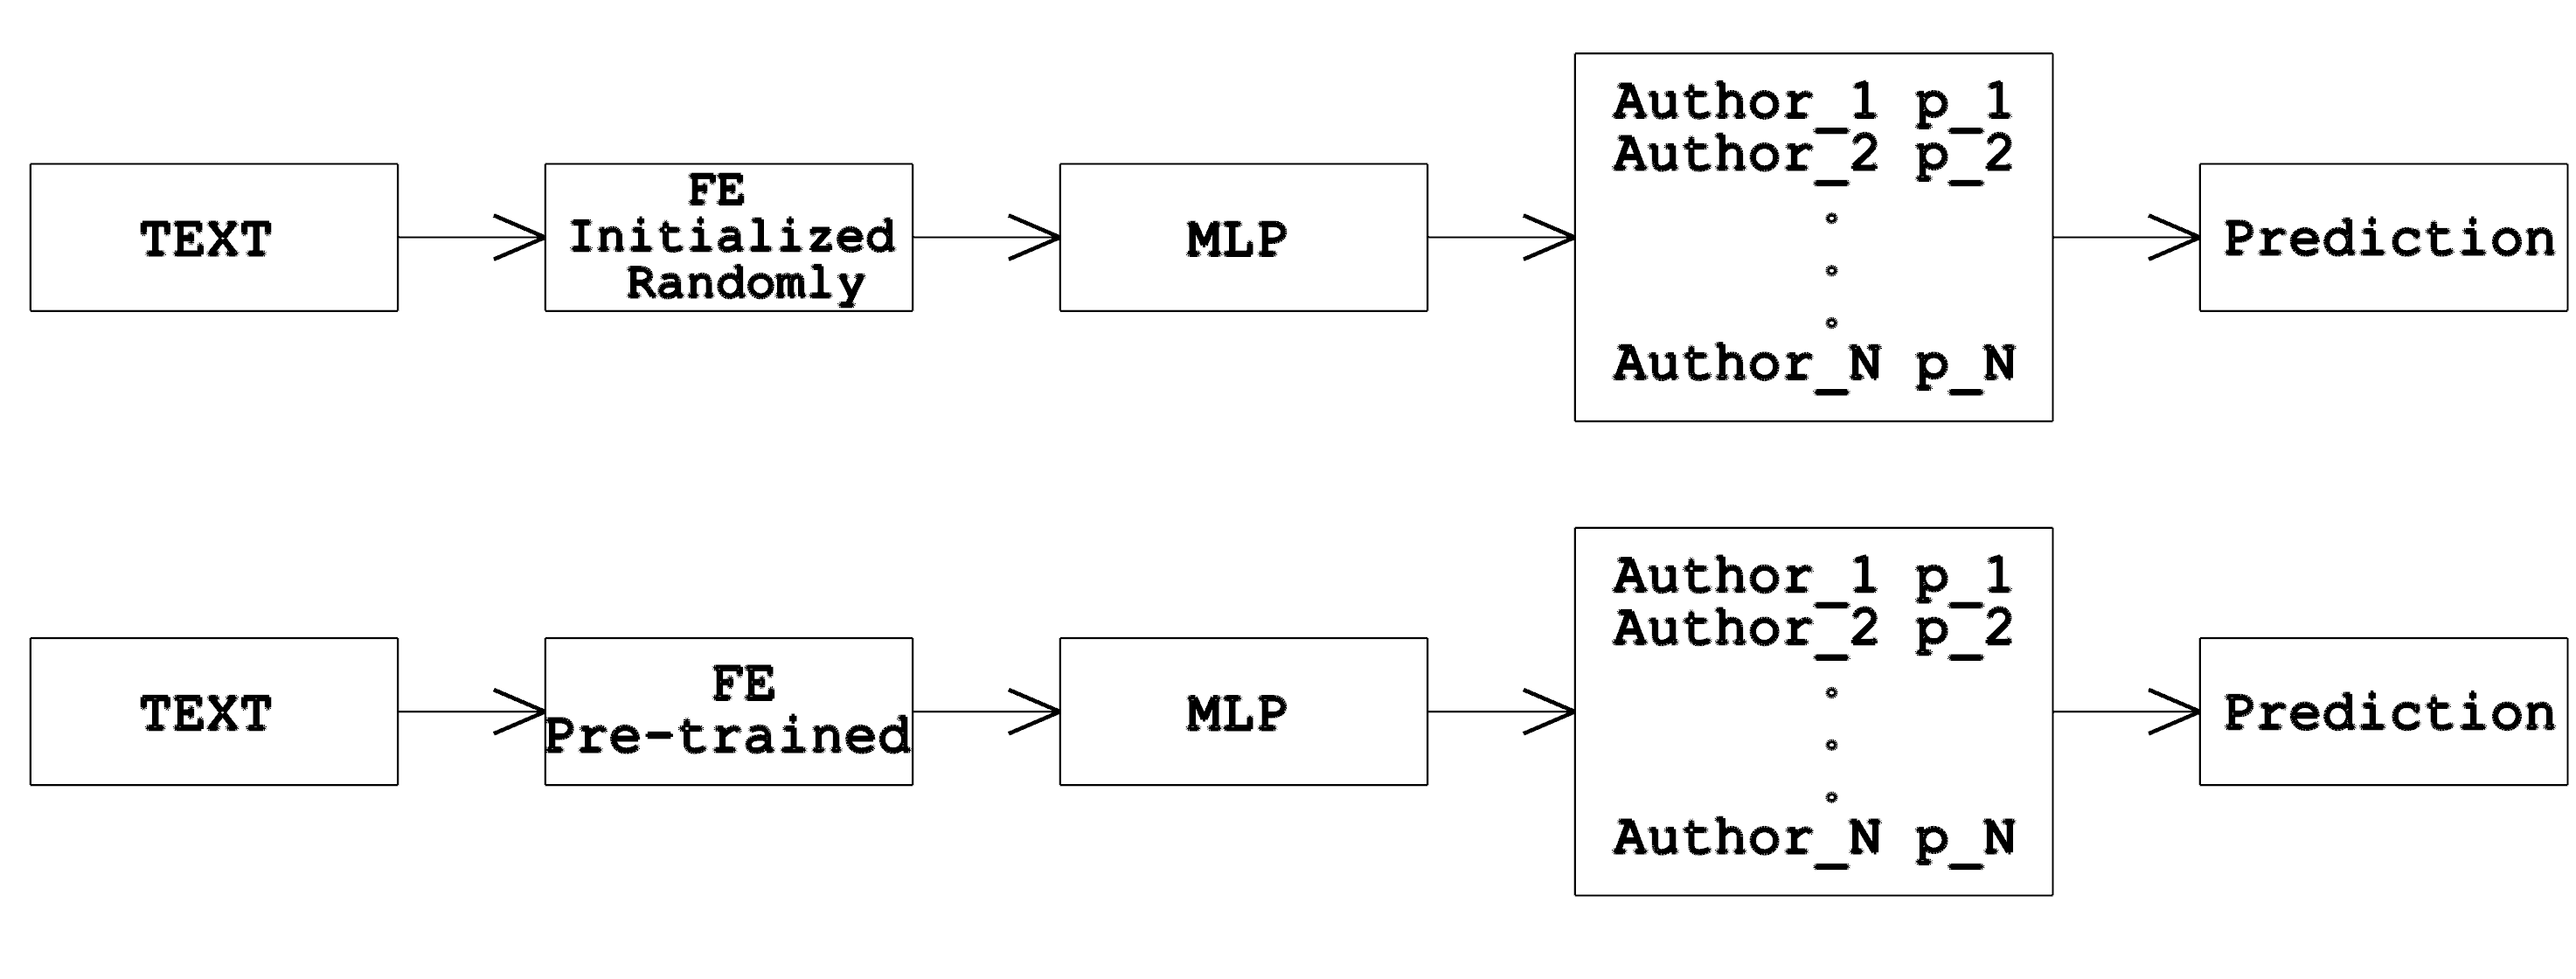
\includegraphics[width=1.0\textwidth]{H1.png}
        \caption{Models for testing the first hypothesis}
\end{figure}

\begin{figure}
  \centering
        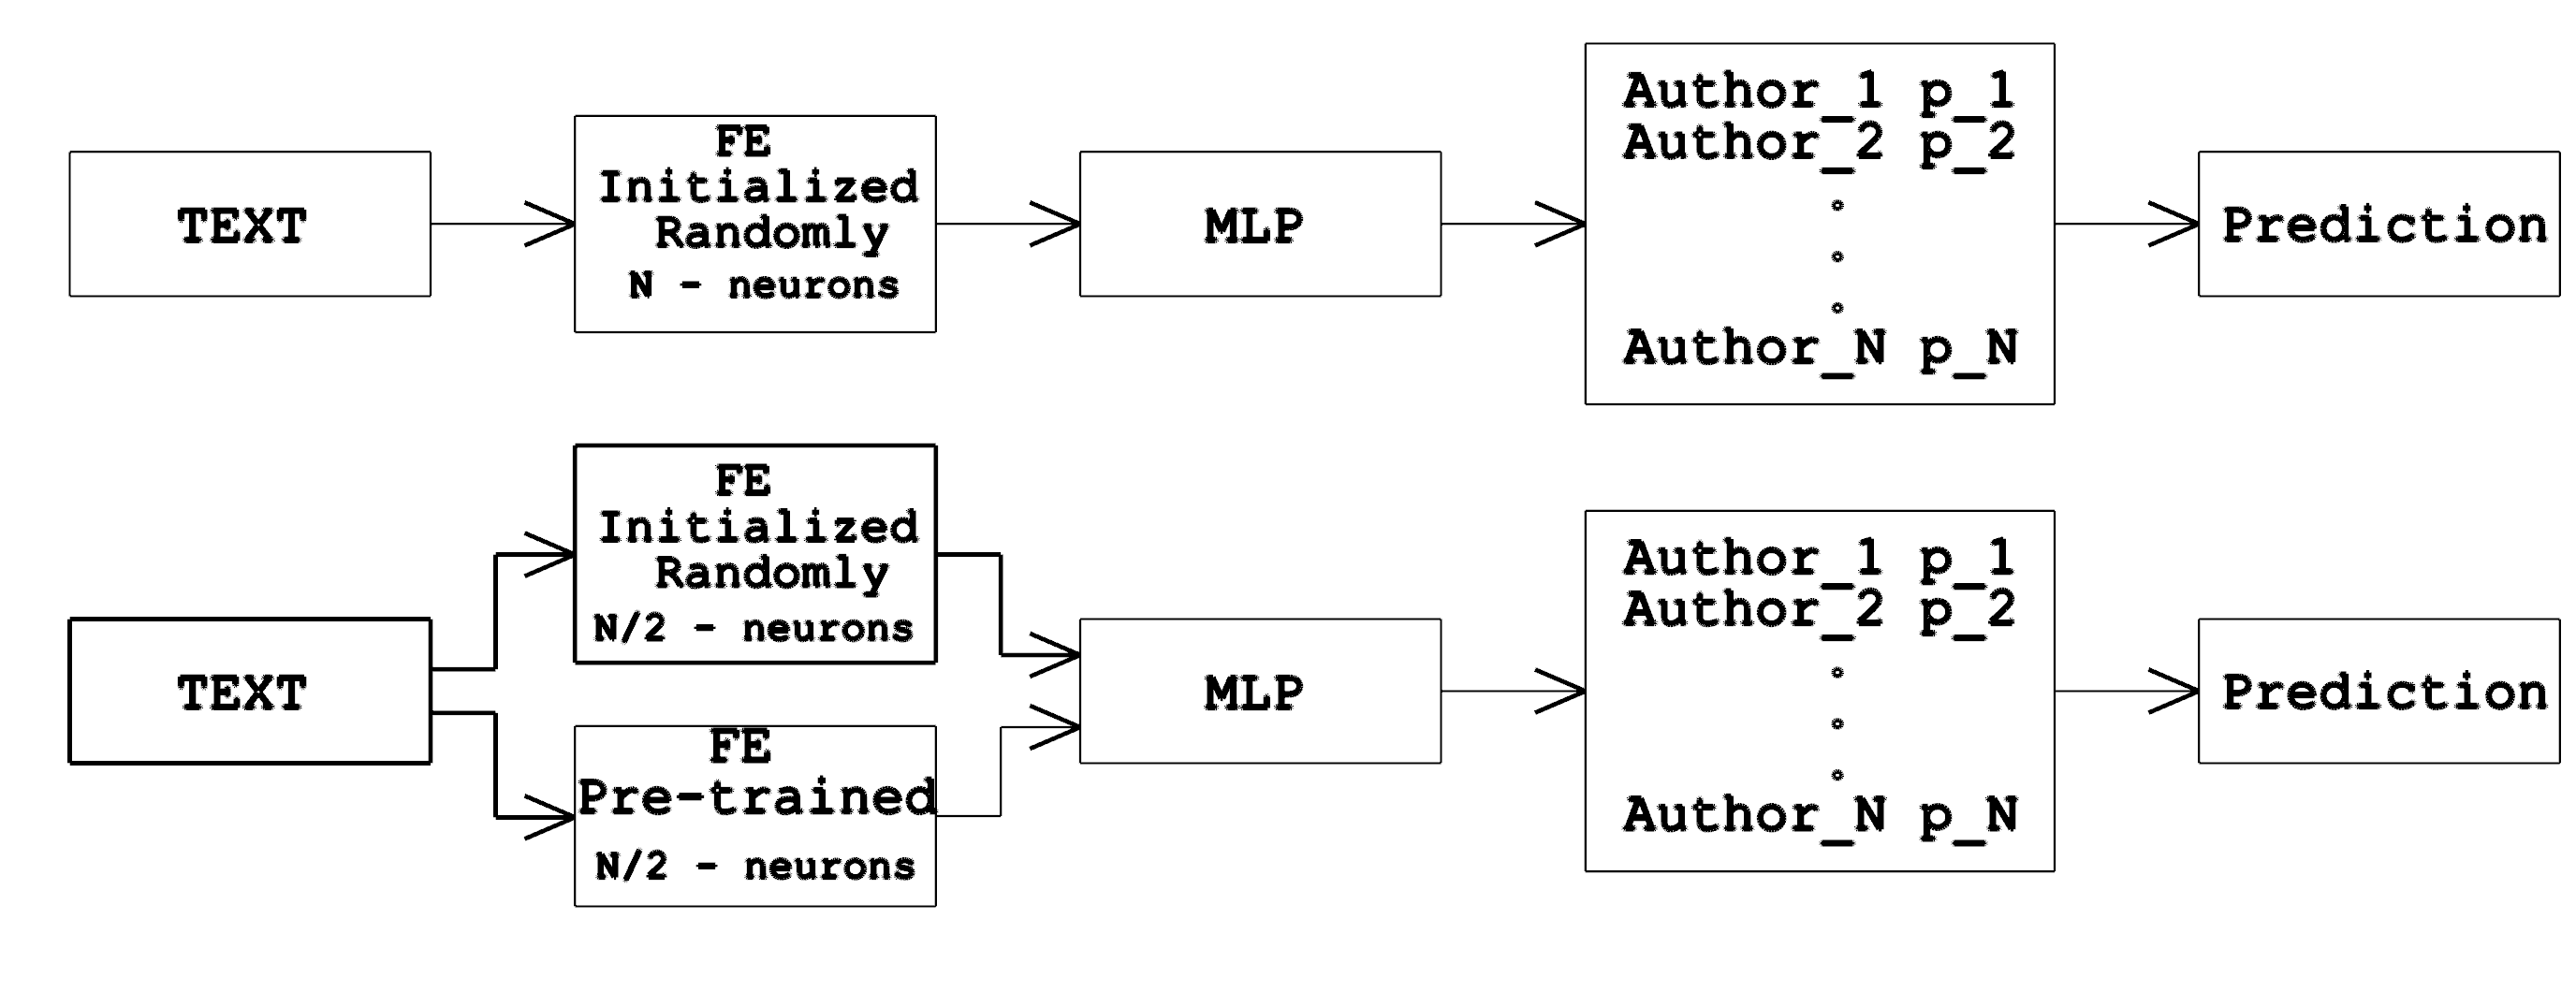
\includegraphics[width=1.0\textwidth]{H2.png}
        \caption{Models for testing the second hypothesis}
\end{figure}

\subsection{Feature extracting model}
As a \textbf{FE} we are considering architectures described on lecture - especially LSTM. It seem to be good baseline model. However concerns me whether it will focus on general task and will specify different style aspect in different output neurons or will it try to solve whole task and MLP will be just a dictionary that maps one author identification embedding into the other. Dropout technique should help, but it might be necessary to consider also different models.


\section{Data, sources and pre-processing}
For the chosen books we are going to look for different translations into English. Some examples
\begin{itemize}
    \item ``Les Miserables''; Victor Hugo; >10 translations into English
    \item ``The Plague''; Albert Camus; >10 translations into English
    \item ``Crime and punishment''; Fyodor Dostoevsky; >10 translations into English
    \item ``The Count of Monte Cristo''; Alexandre Dumas; >10 translations into English
    \item ``Madame Bovary''; Gustave Flaubert; >10 translations into English
    \item ``Bible'' >100 translations into English
\end{itemize}
As input our algorithm takes different versions (translations) of the same text. However, it will be preferable to split it into smaller chunks than whole books. Therefore we consider developing a method for a paragraph to paragraph matching.

List of the English translations of classical literature is meticulously documented ion their corresponding Wikipedia pages. Modern translations have ISBN identifiers assigned which will make it easier to find them on the web. Older translations can be found using more specialised websites, like \href{https://archive.org/}{Internet Archive}.

One of the challenges we have to face will reveal itself right at the beginning, during the data preparation process. We need to collect and match the same sections in each of the translations, this is what constitutes our training data. Because of it, after getting the texts of the translations, we have to develop a matching process. 

At this stage decision has to be made what sections of the text are we going to match. Matching individual sentences seams very unstable, because a translator might decide to split a sentence of the original into multiple in their translation or change the order in which they are presented. 

This encourages us to base matchmaking on a larger section, for example a paragraph. This approach seems more stable, but isn't flawless. Some translations omit whole sections, if their subject is deemed unfitting for the target audience. For example Constance Garnett, when translating "Crime and Punishment" ignored all the parts which she didn't understand. Because of such antics we cannot rely on a simple mapping in the order of appearance.  

Because of it as a part of the data preparation we have to develop a system deciding whether the given paragraphs can be considered the same. The method isn't decided upon, but a set of heuristics comparing length and counting the same words might suffice (of course this requires testing).

\section{Milestone}
Preparing data and training a baseline model.

\section{How will we evaluate success?}
We are considering two methods. First: authorship classification model trained just on given data vs model with the same architecture but with pre-trained feature extraction component (only trainable section is MLP for final classification). The second method will test whether our pre-trained feature extractor will bust the performance of other models.

\section{Relevant existing literature}
\begin{itemize}
    \item \href{https://reader.elsevier.com/reader/sd/pii/S1877050919313791?token=E79C223624500BFB669FF9BACC0506AA22D90F8B15E80D1602653D05322F0E82EFDEB89C5B0597F23413FAE3A29961F2&originRegion=eu-west-1&originCreation=20220524183711}{``A New Method to Identify Short-Text Authors Using Combinations of Machine Learning and Natural Language Processing Techniques''}; Biveeken Vijayakumara, Muhammad Marwan Muhammad Fuadb
    \item \href{https://web.stanford.edu/class/archive/cs/cs224n/cs224n.1174/reports/2760185.pdf}{``Deep Learning based Authorship Identification''}; Chen Qian; Tianchang He; Rao Zhang
\end{itemize}

\end{document}

